\section{Rigid Prototypes}
The goal of this research is to develop a flexible device but before delving into flexible prototypes we started by designing some rigid prototypes. The rigid prototypes were designed to test the concept of the device and to understand the limitations of the technology.

% -- Subsection 2.1
\subsection{1st version - Dresda Coils testbed}
The first prototype was designed to test the capabilities of the Dresden coils.
In the previous research done by the HZDR team \cite{HZDR} they tested the coil using a simple piece of flexible magnetic tape as a membrane.

\subsubsection{Flexible magnetic membrane}
This membrane is shaped like a "fish" so the tail can be fixed on a plane and the head can be free to bend up and down.

\begin{figure}
    \centering
    \resizebox{0.2\textwidth}{!}{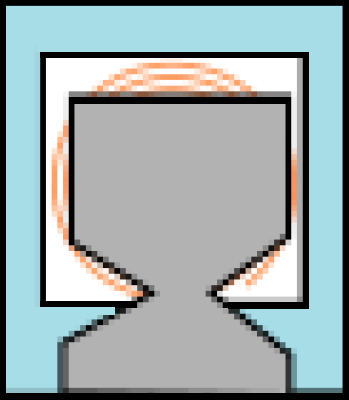
\includegraphics{Chapters/Chapter5/Rigid_Prototypes/Figures/Dresden_test.png}}
    \caption{Dresden coil HZDR test setup}
    \label{fig: Dresden_test}
\end{figure}

When the coil was powered, the magnetic field produced by the coil would repel the membrane and bend it up.
The coil would be powered with an AC signal at various frequencies, then one would need to keep his pulp suspended at a certain distance over the membrane and feel the vibration produced by the membrane.
The pulp needed to be suspended at a certain distance to avoid pressing on the membrane, this would have caused the membrane to stop vibrating.

\subsubsection{Adjustable height platform for coil and membrane}
The most important thing to solve was to find a way to keep the pulp at a certain distance from the membrane.
Firstly we designed a platform that could keep the finger steady.
\begin{figure}
    \centering
    \resizebox{0.5\textwidth}{!}{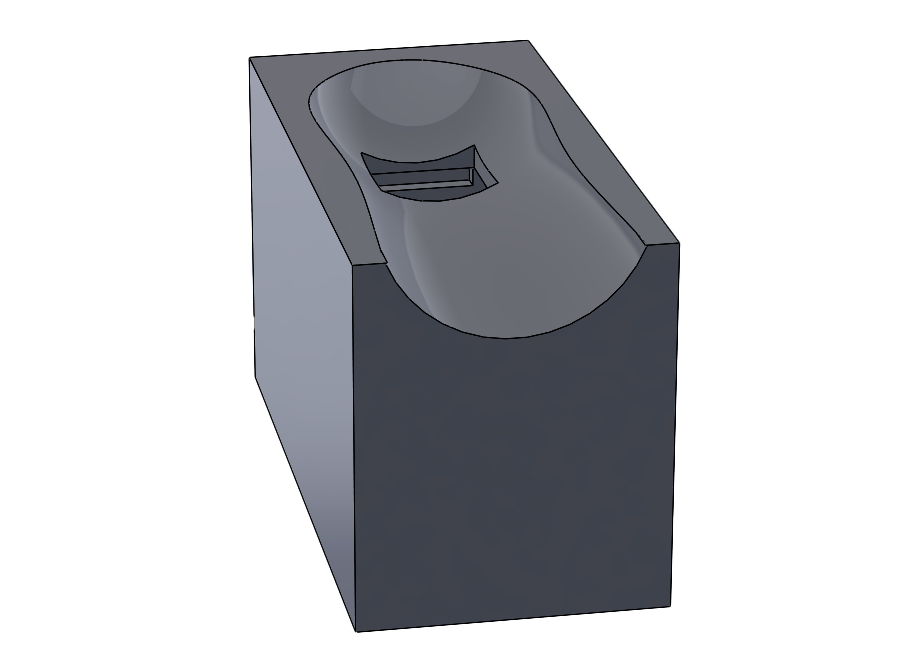
\includegraphics{Chapters/Chapter5/Rigid_Prototypes/Figures/finger_holder.png}}
    \caption{Finger platform}
    \label{fig: finger_platform}
\end{figure}

This platform was modeled to have an ergonomic cavity for the finger to rest in and a hole for the pulp to be suspended over the membrane.
The square hole is large enough to allow the "fish" membrane to move freely.
Under the hole, there is a large cavity where a mechanism is placed.
This mechanism is a platform where the coil and membrane can be placed in a configuration similar to the one used in the HZDR experiment.
The platform can then be raised or lowered to find the right distance between the membrane and the finger pulp.
\begin{figure}
    \centering
    \resizebox{0.5\textwidth}{!}{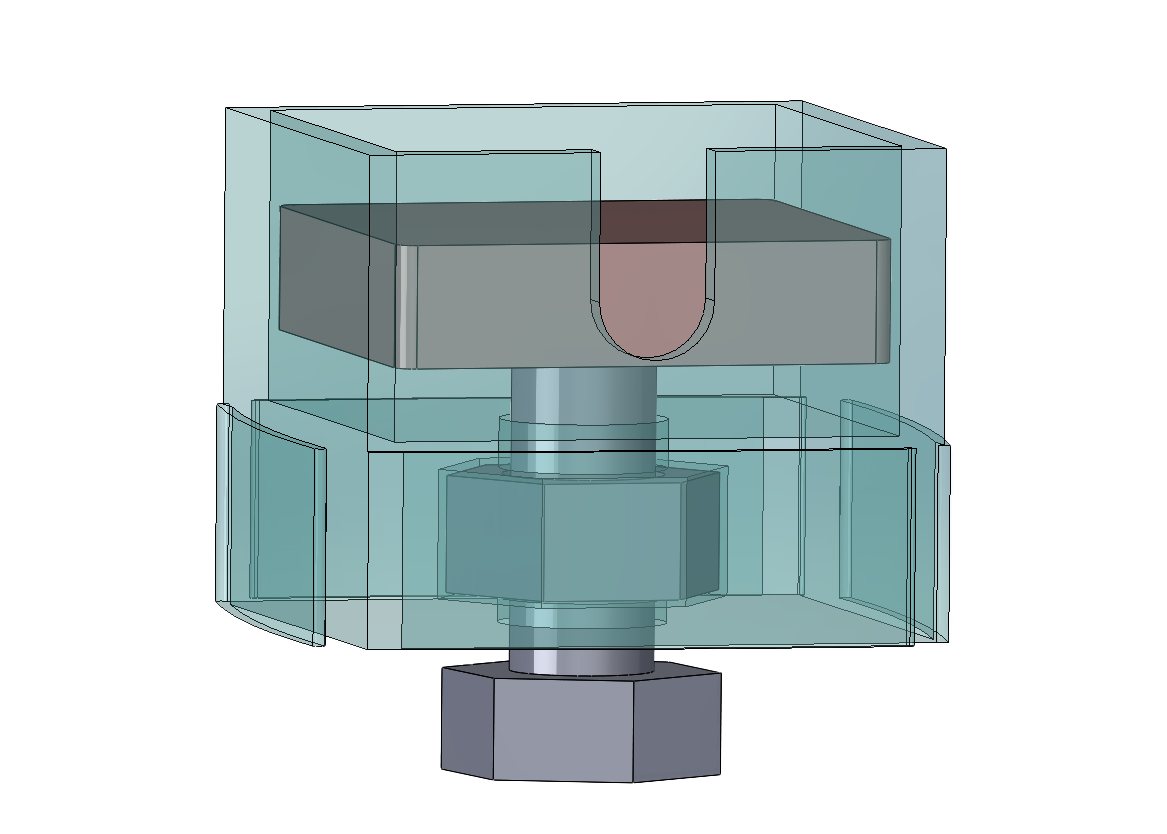
\includegraphics{Chapters/Chapter5/Rigid_Prototypes/Figures/adj_platform.png}}
    \caption{Adjustable platform}
    \label{fig: adj_platform}
\end{figure}
The mechanism is a simple screw that can be turned to raise or lower the platform.

\subsubsection{Prototype usability}
This prototype proved to be pretty finicky to use.
The main problem was that distance couldn't be easily adjusted as the platform wouldn't remain stable enough on the screw.
This meant that finding an optimal distance between the pulp and the membrane was difficult, especially because different people have different pulp thicknesses.
Even if a distance that was good for one person was found, the vibration produced by the membrane was very weak and could barely be felt.

% -- Subsection 2.2
\subsection{Wearable Rigid Prototypes}
With this prototype, we wanted to try fixing most of the problems encountered with the previous prototype.
Firstly we decided to substitute the Dresden coil with the Flexar one as it was more powerful.
Then we wanted to decouple the membrane from the coil to prevent the membrane from being pressed by the pulp and remove the need for an adjustable platform to keep the coil at the right distance.
Finally, we wanted to make the device wearable.

\subsubsection{Finger-Membrane interface}
After some testing, we found that a good way to decouple the membrane from the coil and better the transmission of vibrations to the finger was to use a small high-performance magnet attached directly to the finger pulp.

For our testing, we used an N42-grade neodymium cylindrical magnet with a diameter of \textbf{10mm} and a height of \textbf{3mm}.
This magnet was fixed to the index pulp of the tester using some non-toxic glue and then he would be able to feel substantial vibrations by moving his pulp closer to the powered-on coil (with an AC signal).

Considering this knowledge, we designed a silicon sleeve that could be worn on the finger, this sleeve has a cavity for the magnet to be inserted into and be kept near the skin.
\begin{figure}
    \centering
    \resizebox{1\textwidth}{!}{
        \begin{subfigure}[b]{0.45\textwidth}
            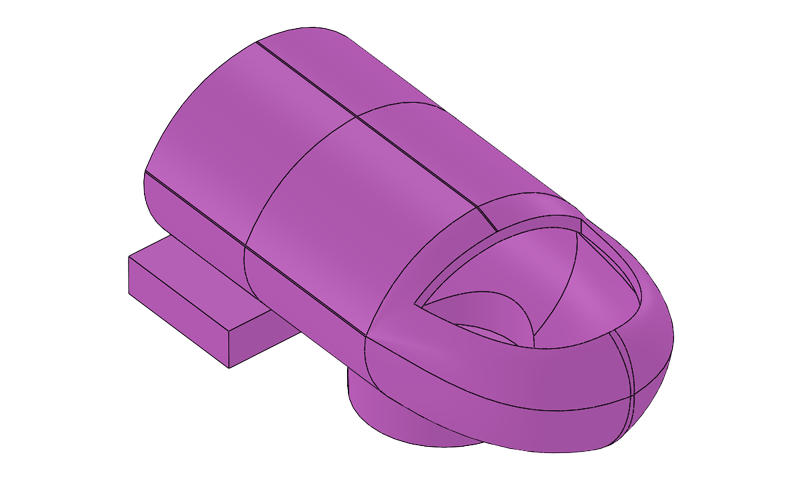
\includegraphics[width=\textwidth]{Chapters/Chapter5/Rigid_Prototypes/Figures/silicon_sleeve_front.png}
        \end{subfigure}
        \begin{subfigure}[b]{0.45\textwidth}
            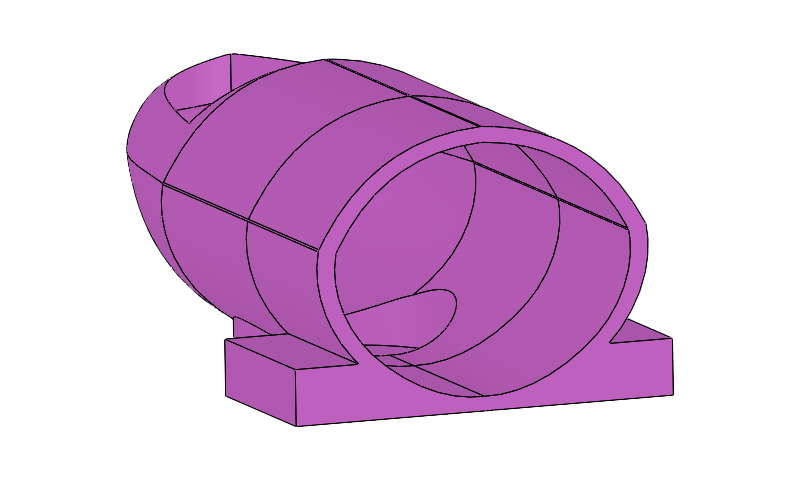
\includegraphics[width=\textwidth]{Chapters/Chapter5/Rigid_Prototypes/Figures/silicon_sleeve_back.png}        
        \end{subfigure}
    }
    \caption{Finger silicon sleeve front and back view}
    \label{fig: finger_sleeve}
\end{figure}

This silicon sleeve was designed to be scalable for different finger sizes and to be easily worn and removed.
The part was produced by silicon casting inside a two-part 3D printed mold.

The design is composed of three parts:
\begin{itemize}
    \item \textbf{Silicon sleeve: } This part was modeled by us on the profile of a real 3d scanned index finger, it can be automatically scaled by specifying the index's width as all the measurements are based on that value.
    \item \textbf{Magnet hole: } The hole is designed based on the diameter of the magnet and its height. We also had to find the right height tolerance between the magnet and the pulp to avoid that it could press on the finger too much, impeding vibrations.
    \item \textbf{Mounting wings: } On the sides of the sleeve we have two parallelepidical wings that are used to mount the sleeve to the structure where the coil will be attached (described in the following section). 
\end{itemize}

Another design problem to solve was the positioning of the magnet, as the design had the goal of being adaptable to different fingertip sizes, we had to consider multiple finger widths. 
For the magnet position we chose the center to be placed on the symmetry axis of the pulp, then we based the design on index fingers with widths between \textbf{13mm} and \textbf{20mm} \cite{index_fingers_width}.
That meant that for 13mm fingers, the magnet size (10mm) was barely smaller than the finger's width, so knowing that the finger tends to get even narrower toward the tip, we had to place the magnet center closer to the first interphalangeal fold rather than to the pulp's center.

\subsubsection{Sleeve production}
The sleeve was produced by silicon casting inside a two-part 3D printed mold:
\begin{itemize}
    \item \textbf{Mold cavity: } The cavity was designed based on the 3D model of an index finger, with the addition of a small surface to produce the opening for the fingernail (the part in grey in figure \ref{fig: mold_cavity})and half of the hole necessary to create the magnet cavity.
    \begin{figure}
        \centering
        \resizebox{0.5\textwidth}{!}{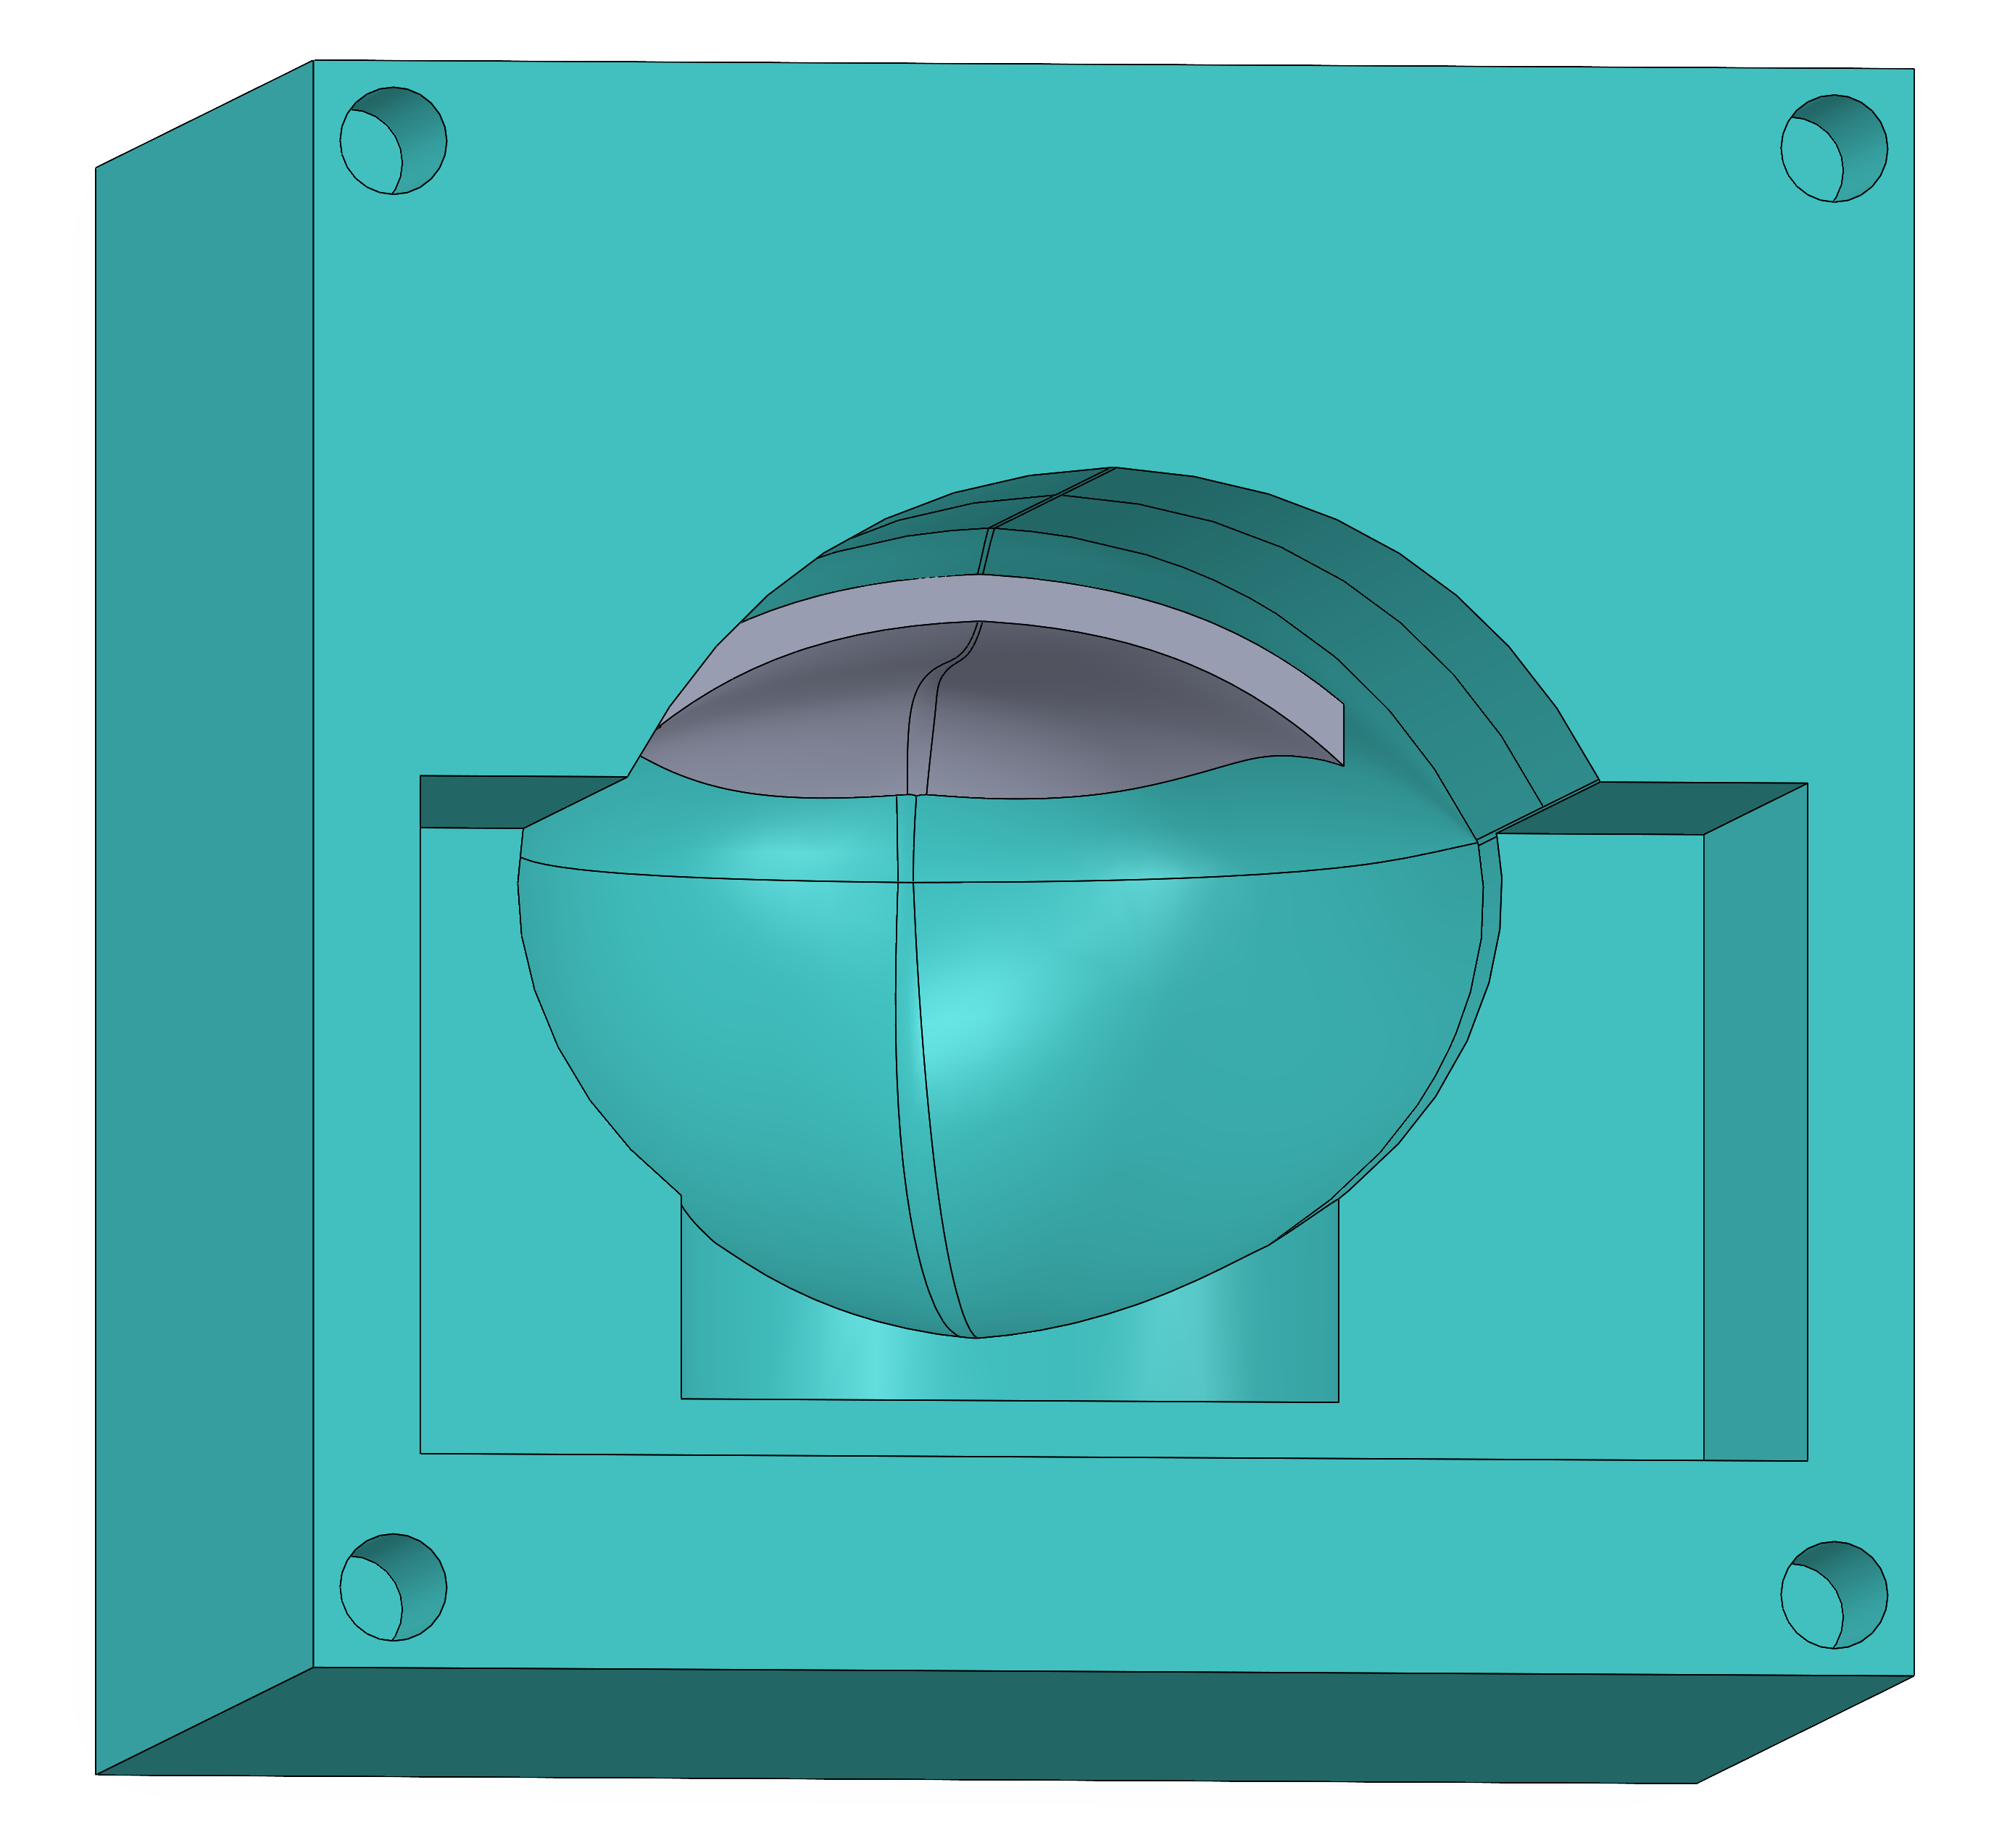
\includegraphics{Chapters/Chapter5/Rigid_Prototypes/Figures/silicon_finger_mold_cavity.PNG}}
        \caption{Mold cavity}
        \label{fig: mold_cavity}
    \end{figure}

    \item \textbf{Mold core: } The core was designed to be the negative of the cavity, including a part to create the other half of the magnet cavity and mounting wings (the part in light blue in figure \ref{fig: mold_core}).
    The negative is scaled down a bit to create a casting clearance of about 0.8mm.
    This part also includes a cap that is screwed on the cavity to keep the core suspended in the silicon.
    \begin{figure}
        \centering
        \resizebox{0.5\textwidth}{!}{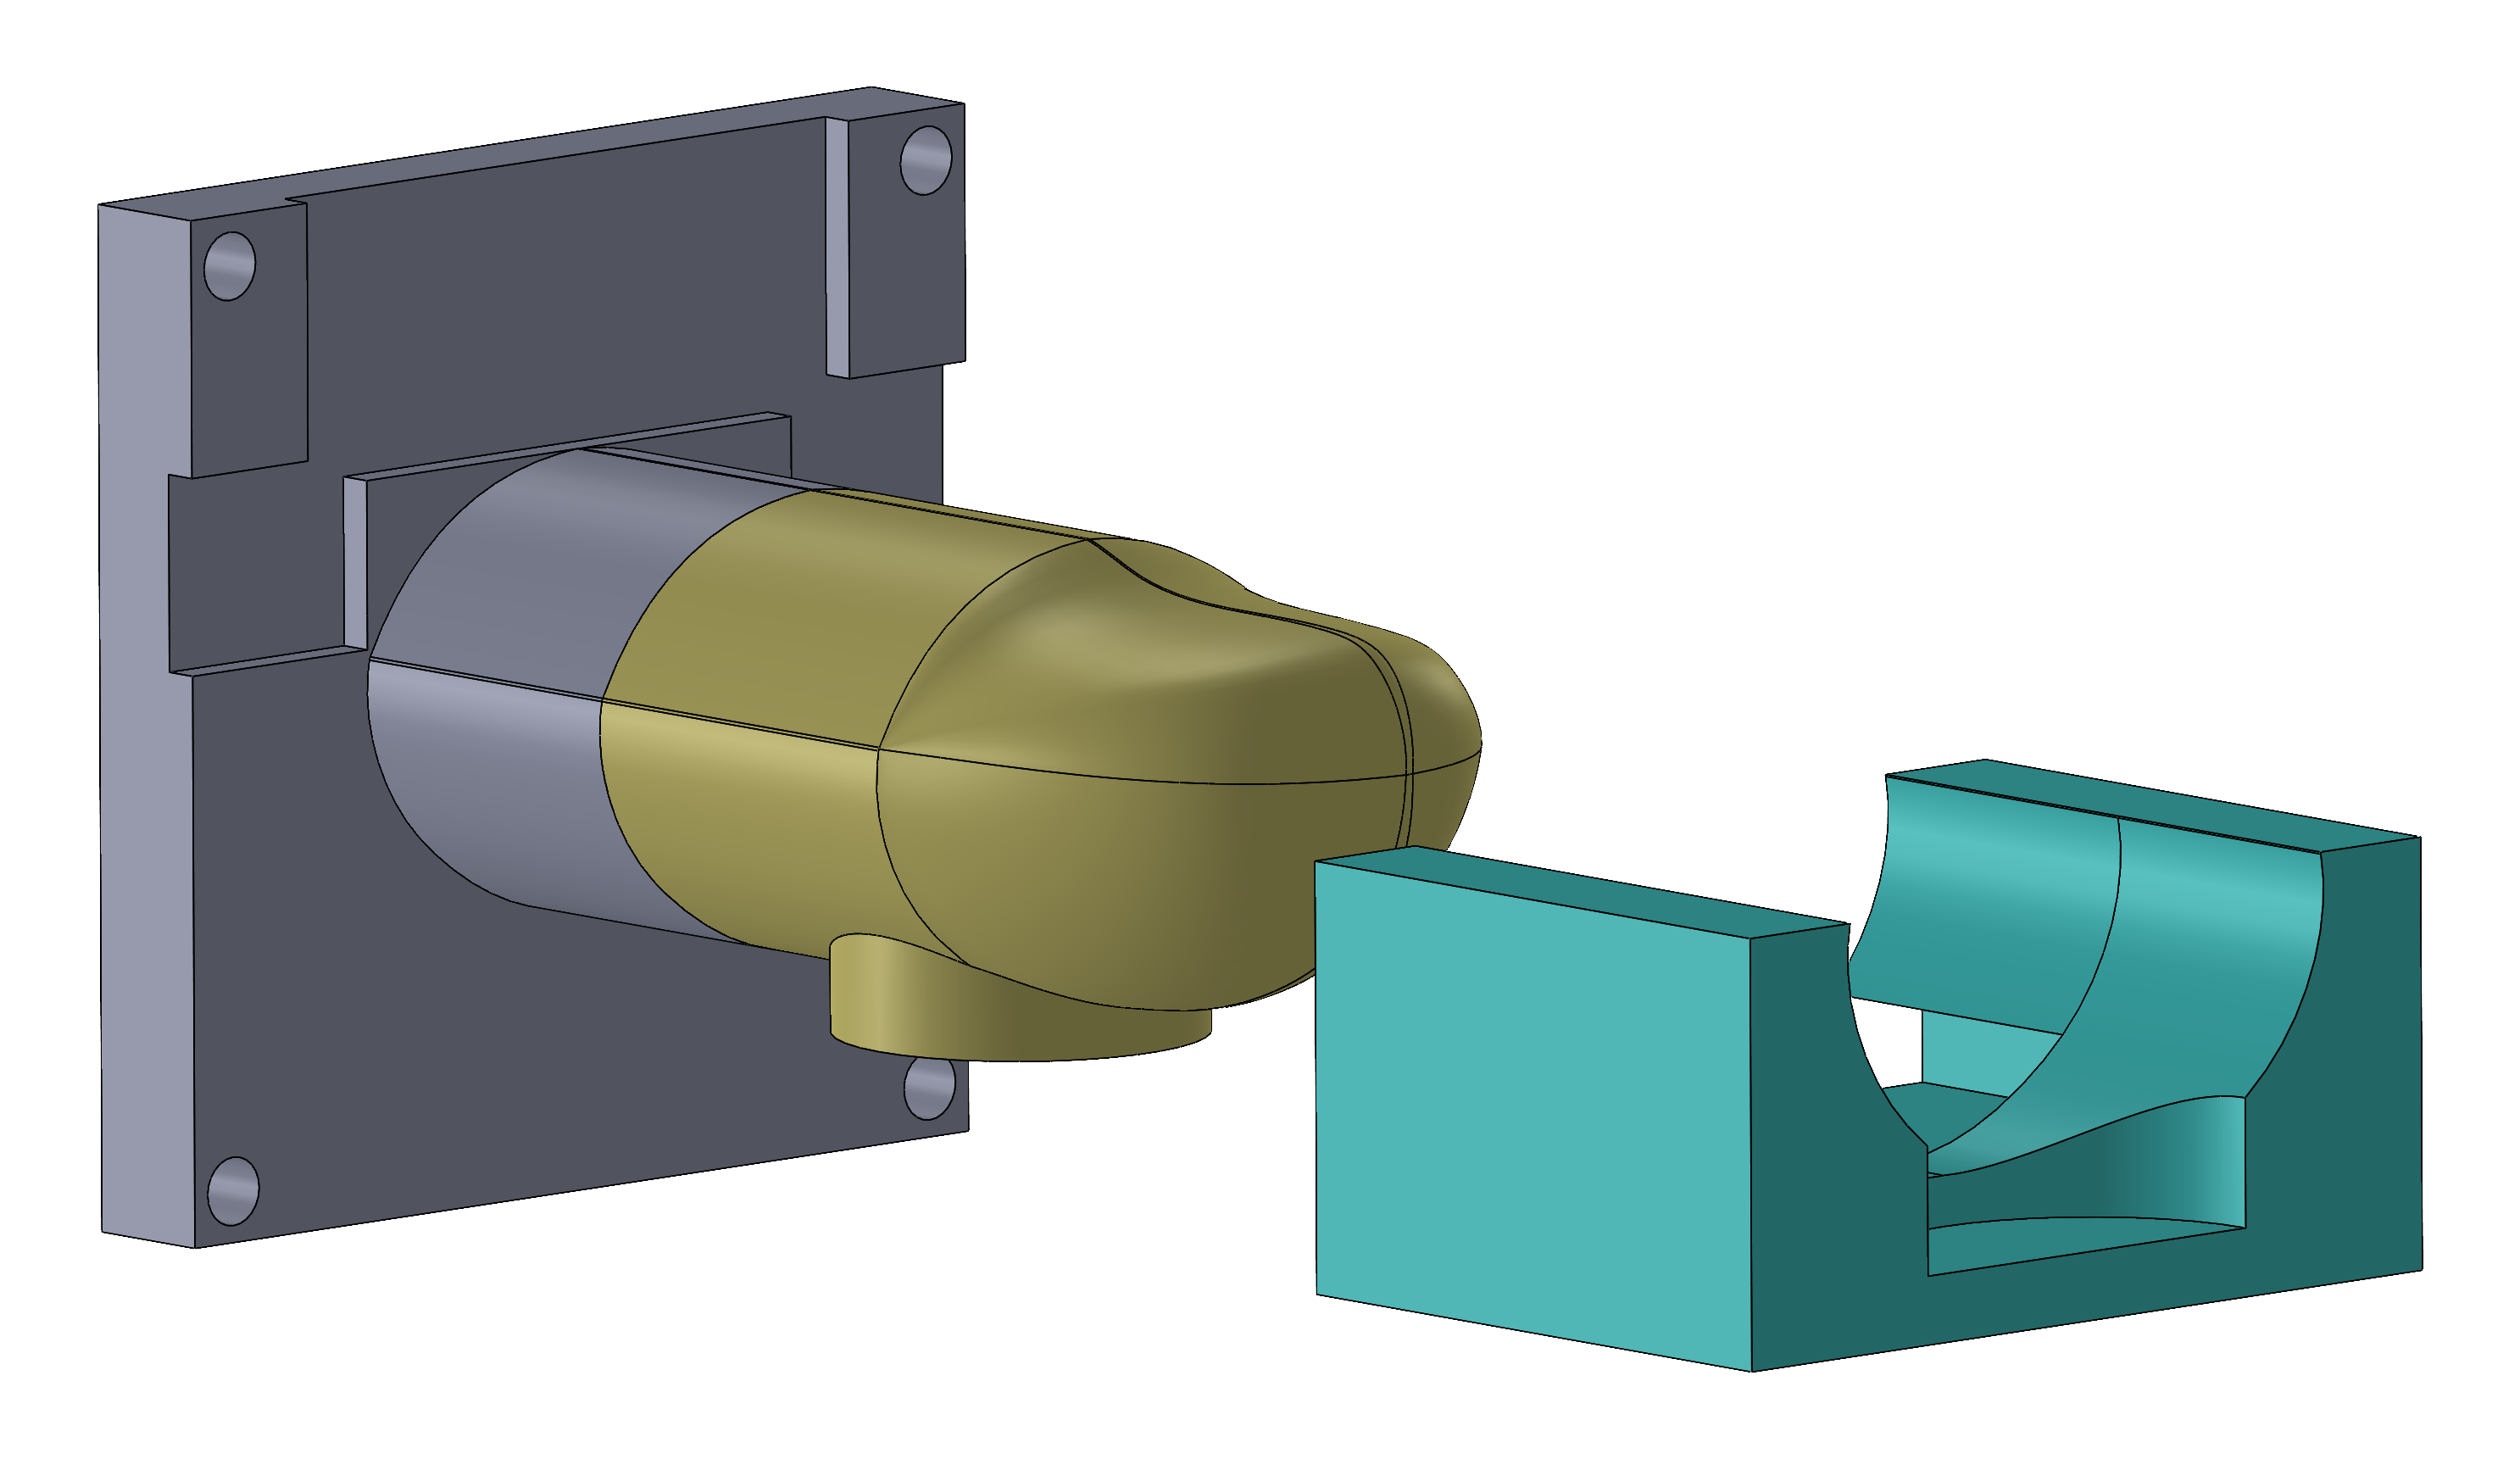
\includegraphics{Chapters/Chapter5/Rigid_Prototypes/Figures/silicon_finger_mold_core.PNG}}
        \caption{Mold core}
        \label{fig: mold_core}
    \end{figure}
\end{itemize}

The part went through multiple iterations to land on the right thicknesses for the sleeve itself, it needed to be thin enough to be adaptable to multiple fingers (considering similar widths) but not so thin as to be durable enough.

The material used for the casting was a two-component silicon rubber from ResChimica.
We tested two different types of silicon, one with a shore hardness of 12 \cite{R_Pro_10_silicon} and one with a shore hardness of 35 \cite{R_Pro_Fast_silicon}.

From our tests, we found that the silicon with a shore hardness of 35 was too rigid and absorbed too much vibration so we decided to use the softer one.
The only problem with this softer silicon was its minimum curing time of 3 hours at room temperature which always had to be increased as it never cured completely in that time.

\subsubsection{Keep the distance from the coil}
We then focused on a structure able to keep the coil at a fixed distance from the silicon sleeve and magnet.
The design goals for this device were that it should be lightweight, easily wearable and adaptable to multiple sleeves' sizes.

\begin{figure}
    \centering
    \resizebox{1\textwidth}{!}{
        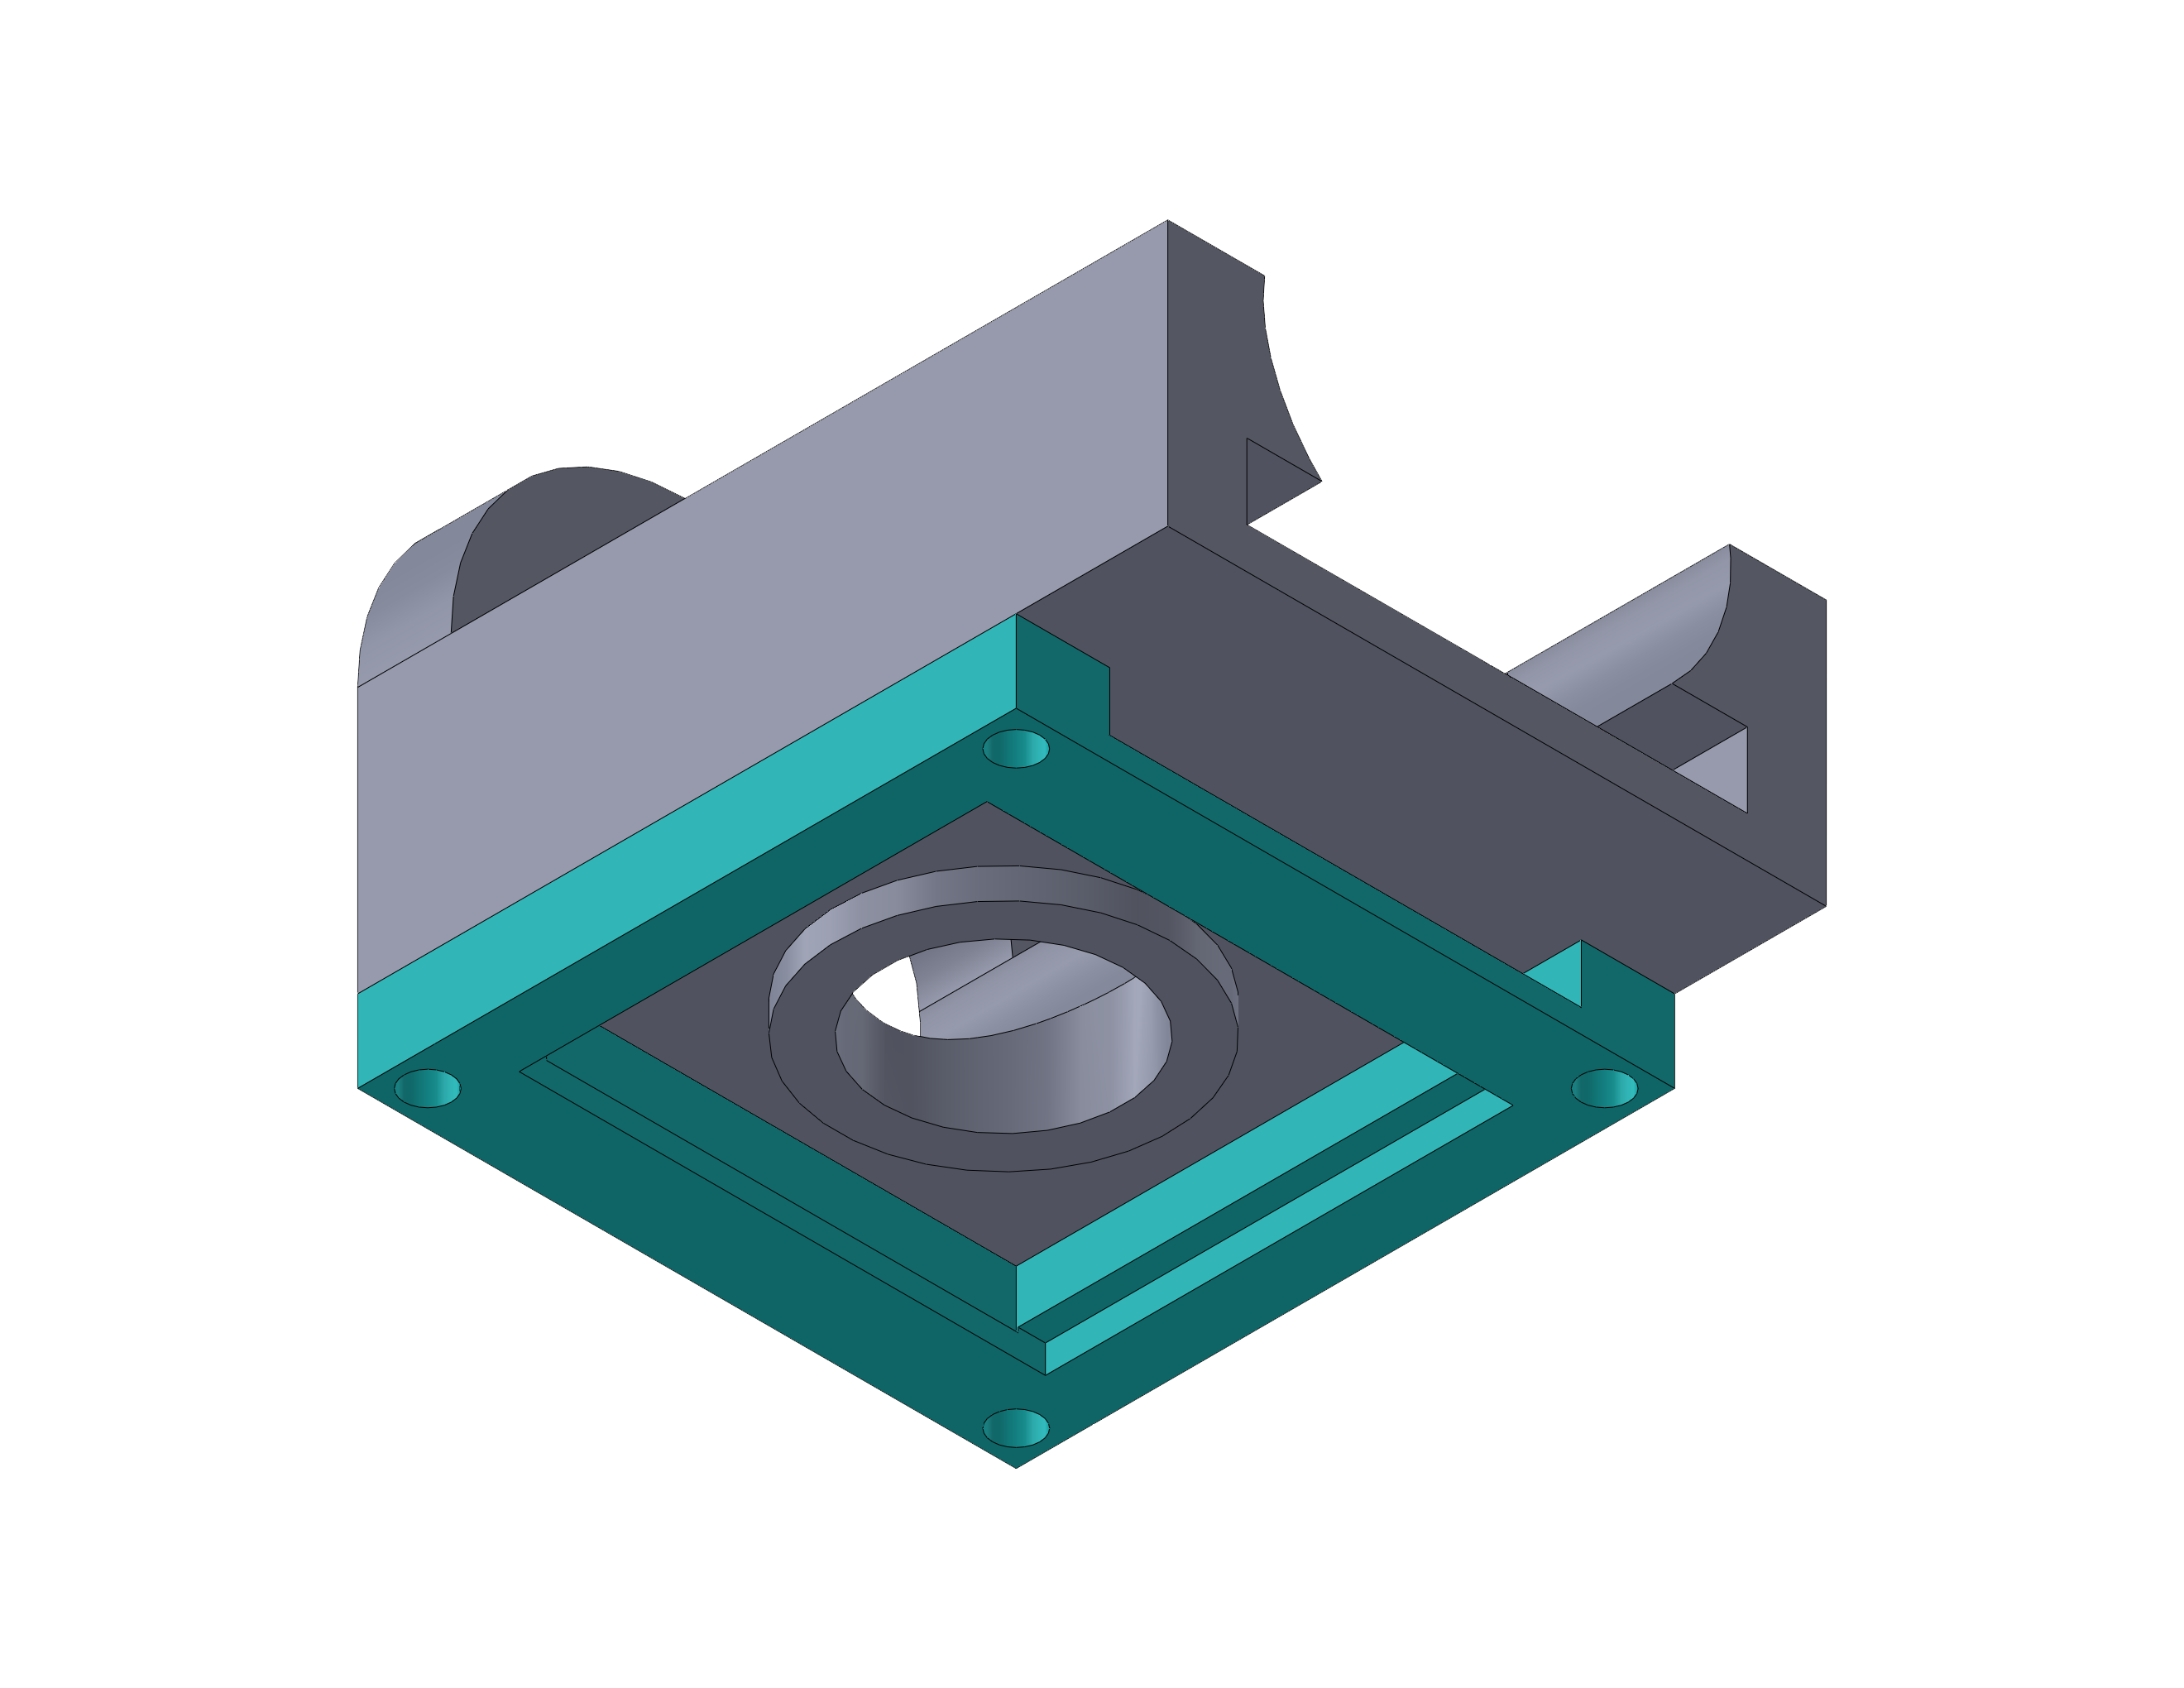
\includegraphics{Chapters/Chapter5/Rigid_Prototypes/Figures/sleeve_holder_complete.png}
    }
    \caption{Explode of the complete silicon finger sleeve holder}
    \label{fig: sleeve_holder_complete}
\end{figure}

After multiple iterations, we landed on a three-component design.
\begin{itemize}
    \item \textbf{Sleeve holder: } This component is the structure where the sleeve can be attached, this is done by inserting the mounting wings inside the two squared holes on the bottom of the part.
    The circle hole at the center of the component is where the magnet cavity of the sleeve with the magnet inside will be placed.
    The arch on the component front is present to allow the tip of the finger to support the weight of the structure.
    \begin{figure}
        \centering
        \resizebox{1\textwidth}{!}{
            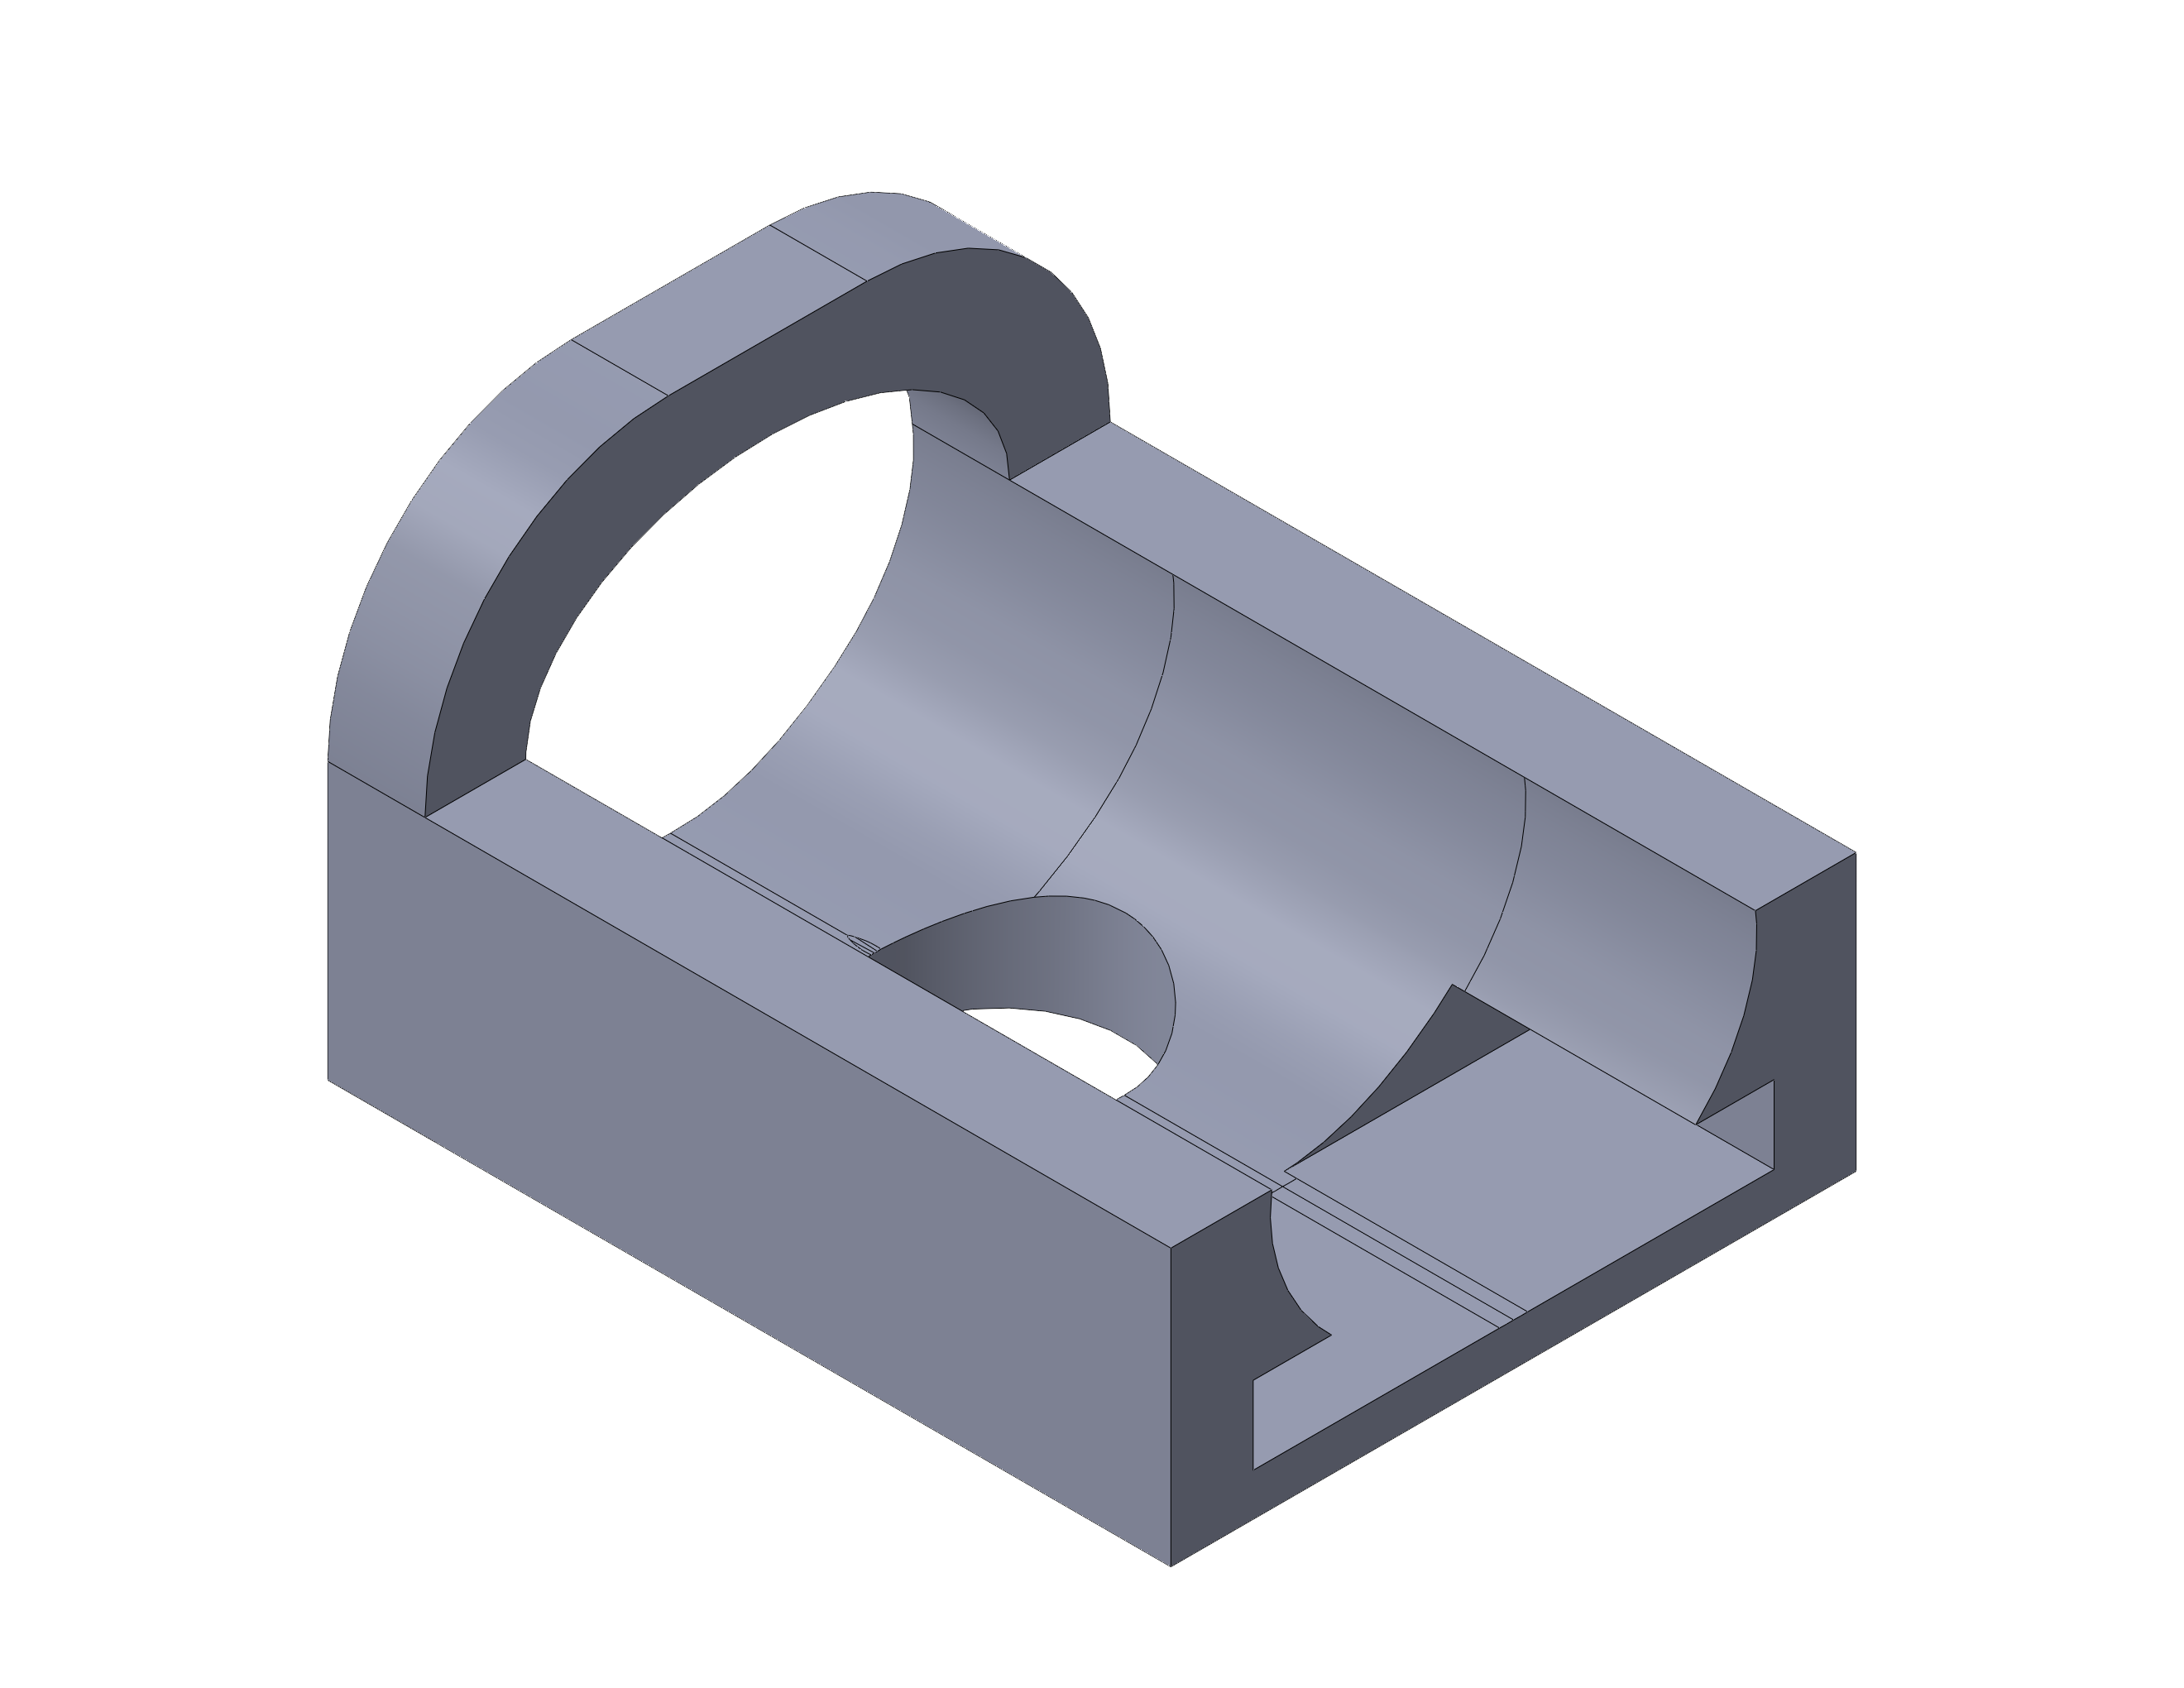
\includegraphics{Chapters/Chapter5/Rigid_Prototypes/Figures/sleeve_holder.png}
        }
        \caption{Silicon finger sleeve holder}
        \label{fig: sleeve_holder}
    \end{figure}

    \item \textbf{Coil trap: } This component is the structure where the coil is inserted. This component is composed of 3 parts, a heatsink, a coil holder and a mask to screw the heatsink to the sleeve holder.
    The coil is sandwiched between the heatsink (the part in bronze) and the coil holder (the part in grey). Then they are screwed together to the sleeve holder.
    \begin{figure}
        \centering
        \resizebox{1\textwidth}{!}{
            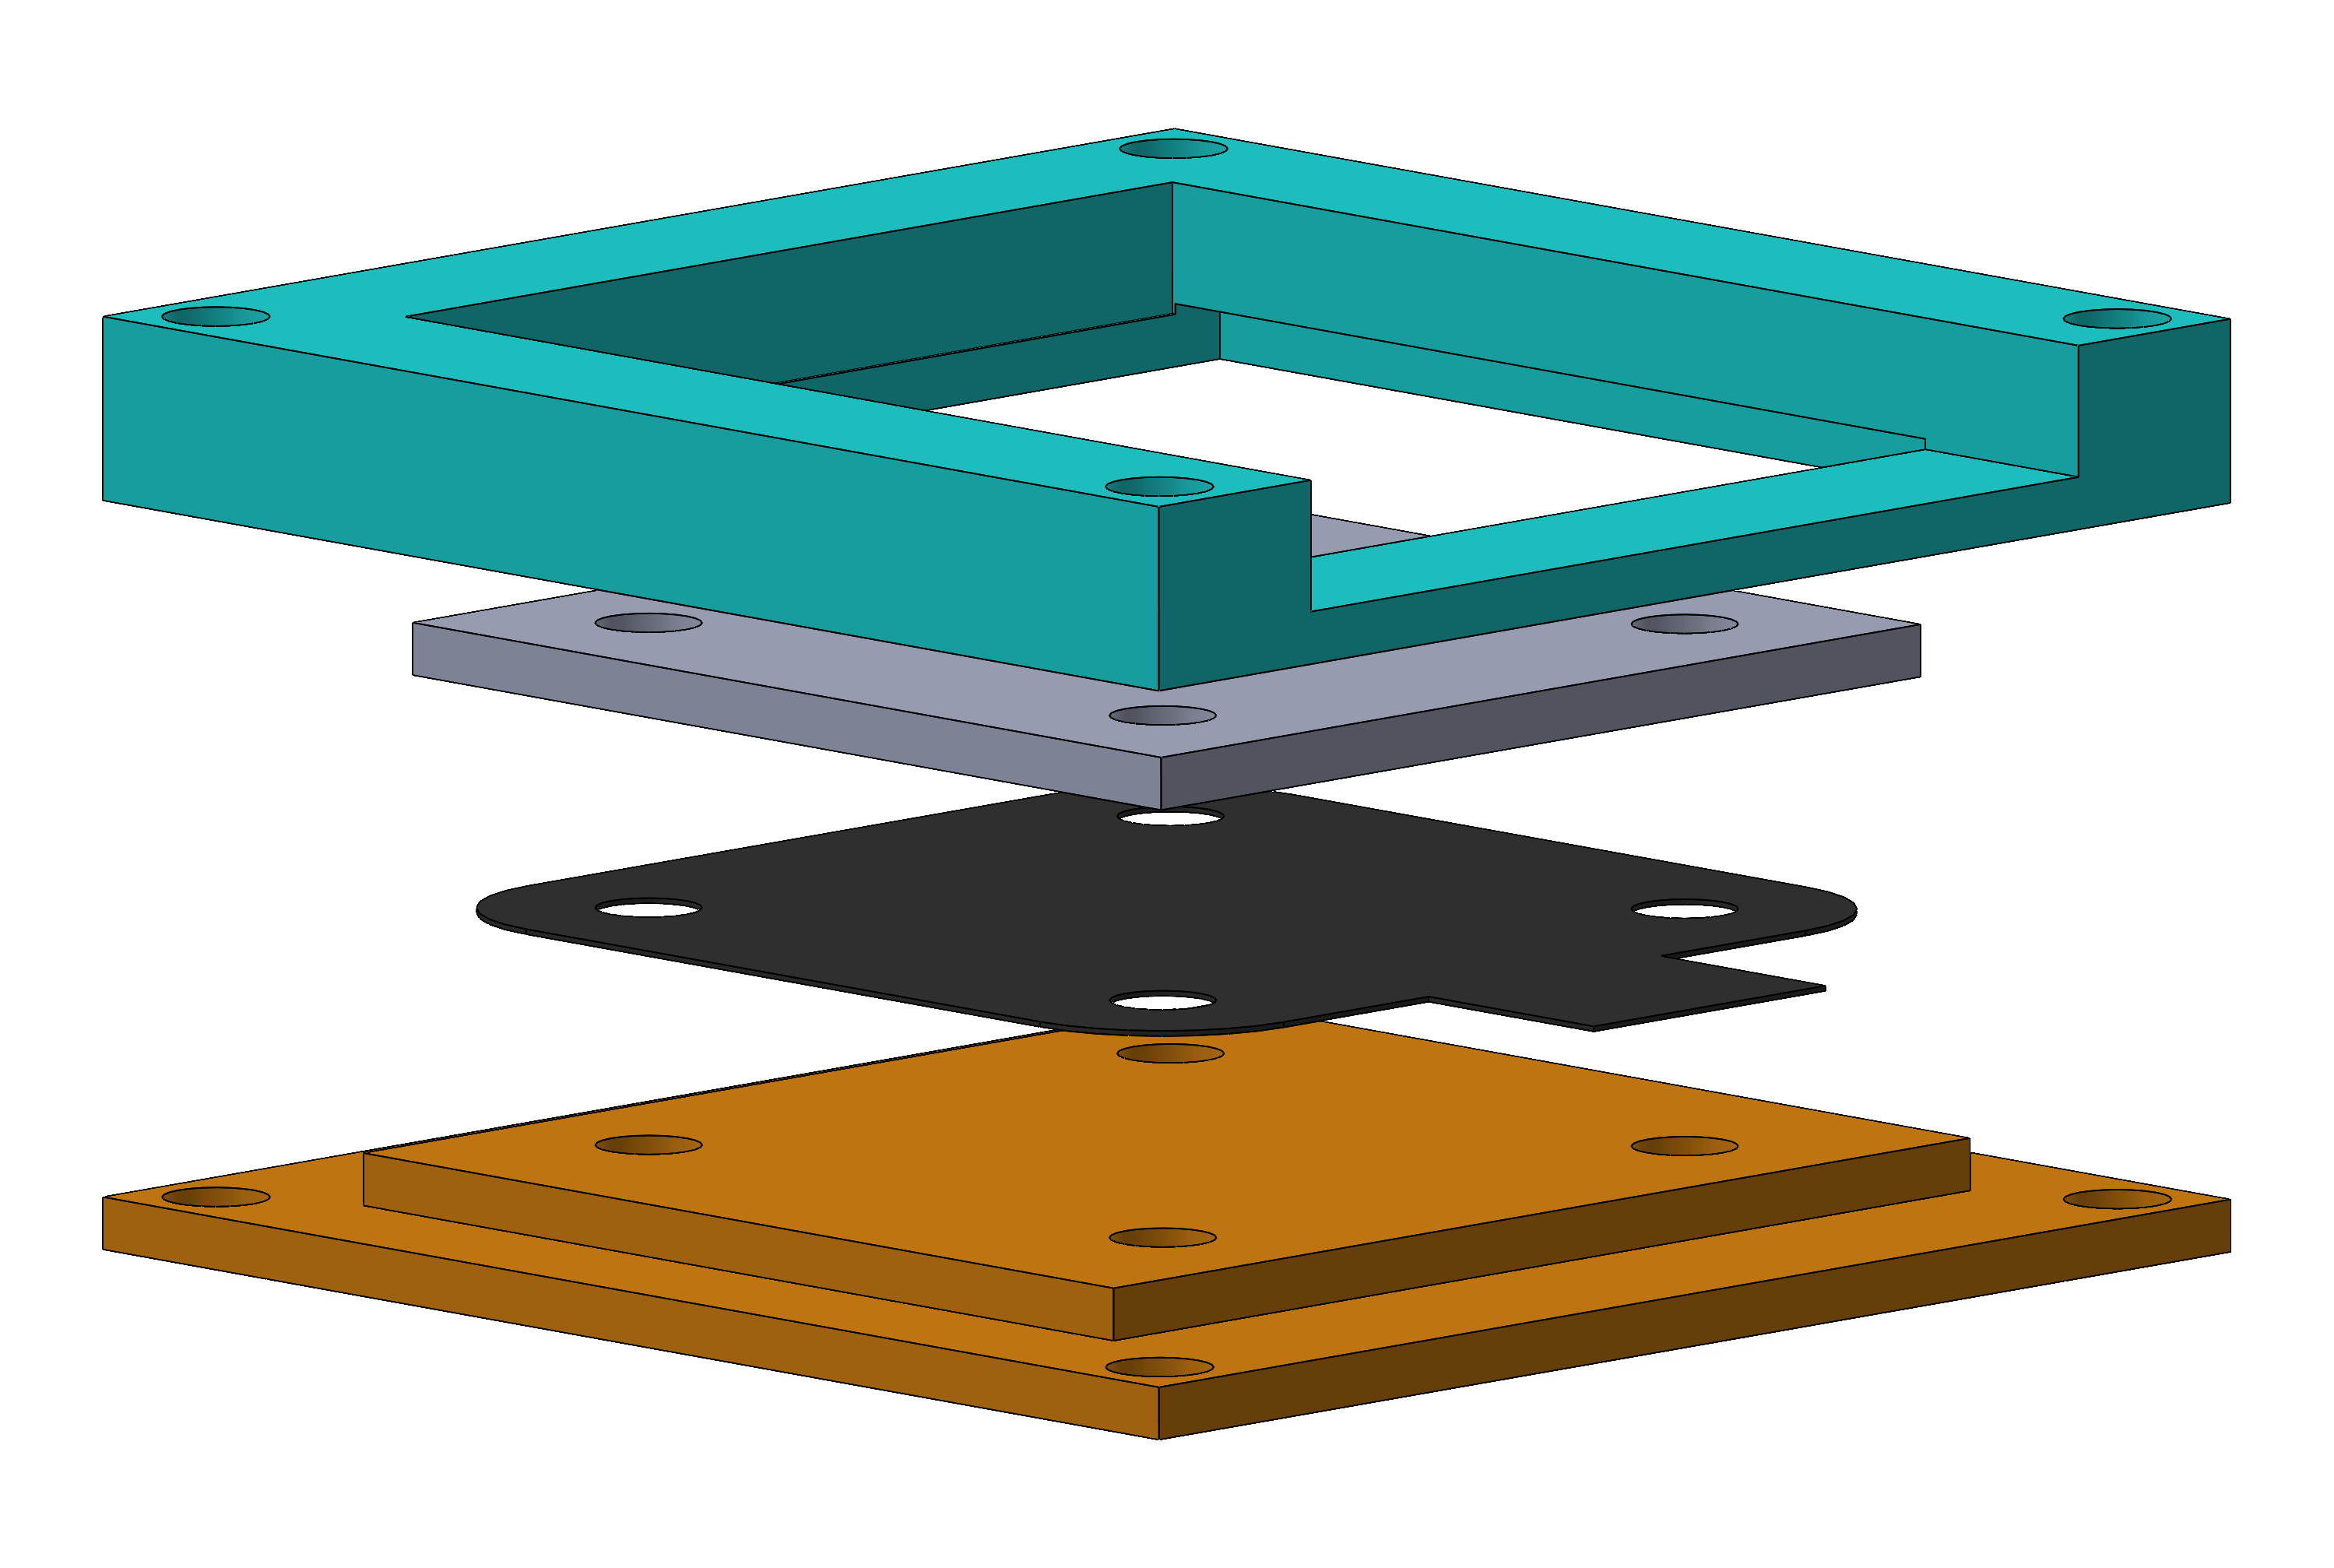
\includegraphics{Chapters/Chapter5/Rigid_Prototypes/Figures/coil_trap.png}
        }
        \caption{Explode of the coil trap}
        \label{fig: coil_trap}
    \end{figure}
    
\end{itemize}

\subsubsection{Heat dissipation}
As the coil while active produces a lot of heat, we decided to introduce a heatsink in the design (the part in bronze in figure \ref{fig: coil_trap}).
The heatsink was made by cutting two small strips from a thin sheet of copper (1mm thick) that are joined together by thermal paste and screws.
The same screws are also used to keep in place the coil and the coil holder.

For the same heat dissipation reason, we printed all components in ABS as it has a higher melting point than PLA.

\subsubsection{Prototype usability}
This prototype was much more usable than the previous one.
The magnet was also kept at the right distance from the coil and the vibrations were much more noticeable, also being wearable made it much easier to use.
The biggest problem of this prototype was the silicon sleeve, as the silicon tends to absorb some of the vibrations produced by the coil and the softness of the material made the mounting mechanism a bit finicky.
We also had to add a small blowing fan and another part to the heatsink (as we can see in figure \ref{fig: rigid_prot}) to keep the coil cool as it would heat a lot after a few minutes of use.

\begin{figure}
    \centering
    \resizebox{1\textwidth}{!}{
        \begin{subfigure}[b]{0.45\textwidth}
            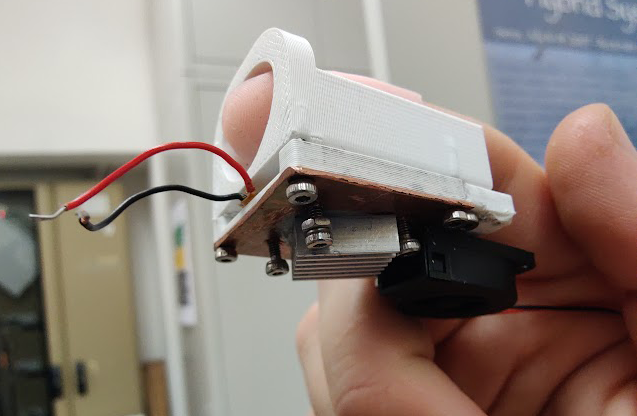
\includegraphics[width=\textwidth]{Chapters/Chapter5/Rigid_Prototypes/Figures/rigid_prot_btm.png}
        \end{subfigure}
        \begin{subfigure}[b]{0.45\textwidth}
            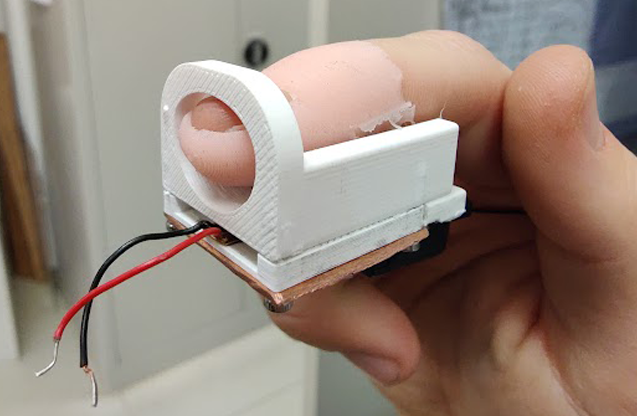
\includegraphics[width=\textwidth]{Chapters/Chapter5/Rigid_Prototypes/Figures/rigid_prot_top.png}        
        \end{subfigure}
    }
    \caption{Bottom and top view of the real prototype}
    \label{fig: rigid_prot}
\end{figure}

